% How X-Forge works. Build: tectonic how-it-works.tex (or pdflatex), then
%   dvisvgm --pdf how-it-works.pdf -o how-it-works.svg
\documentclass[tikz,border=8pt]{standalone}
\usepackage[T1]{fontenc}
\usepackage{lmodern}
\usetikzlibrary{positioning,arrows.meta,fit,backgrounds}

\definecolor{agent}{HTML}{DCE9F7}  \definecolor{agentline}{HTML}{3A6EA5}
\definecolor{code}{HTML}{E4F2DF}   \definecolor{codeline}{HTML}{4A7F3A}
\definecolor{io}{HTML}{F2F2F2}     \definecolor{ioline}{HTML}{777777}

\tikzset{
  base/.style={rounded corners=3pt, minimum height=11mm, text width=24mm, align=center,
               font=\sffamily\small, line width=0.8pt},
  agent/.style={base, fill=agent, draw=agentline},
  code/.style={base, fill=code, draw=codeline},
  io/.style={base, fill=io, draw=ioline, text width=26mm},
  flow/.style={-{Stealth[length=2.2mm]}, line width=0.8pt, draw=black!70},
  back/.style={flow, dashed},
  lane/.style={draw=black!25, rounded corners=6pt, inner sep=5mm},
  title/.style={font=\sffamily\bfseries, anchor=south west},
  note/.style={font=\sffamily\scriptsize, text=black!65, align=center},
}

\begin{document}
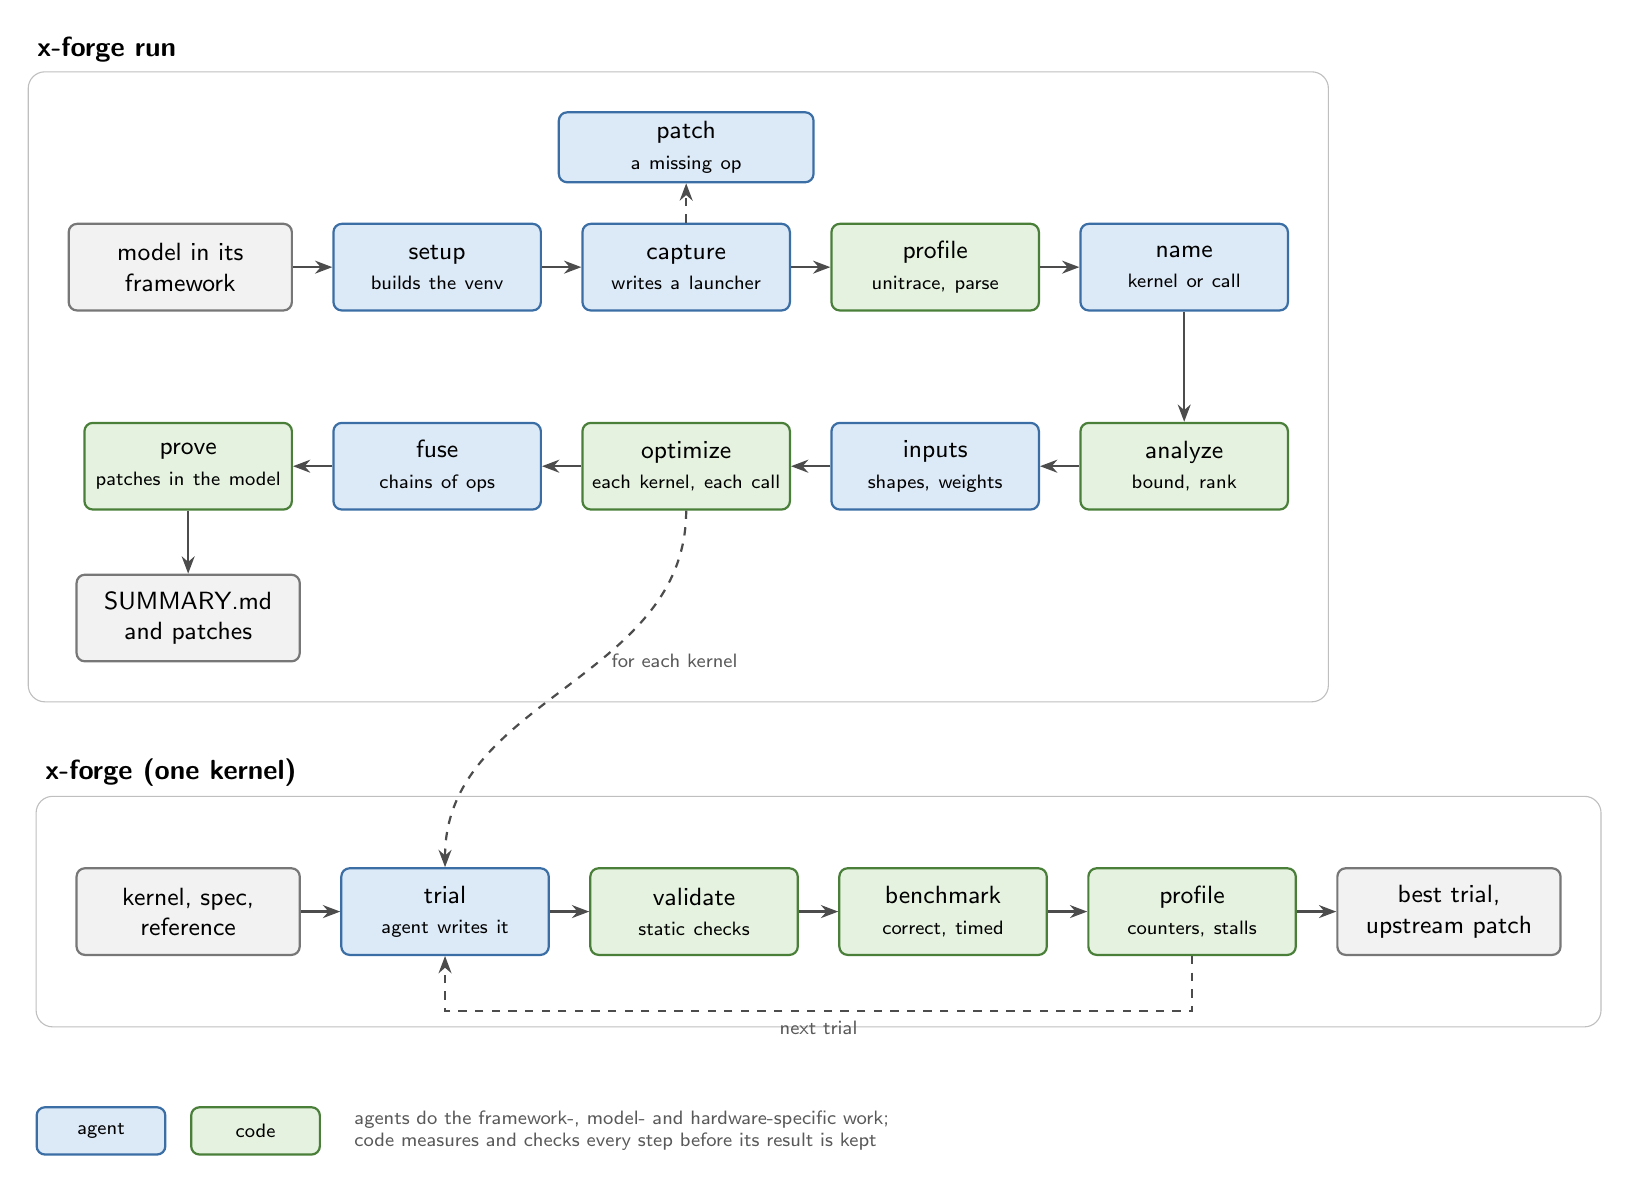
\begin{tikzpicture}[node distance=6mm and 5mm]

% ---- x-forge run: a model in its framework ----
\node[io]    (model)  {model in its\\framework};
\node[agent, right=of model]  (setup)  {setup\\\scriptsize builds the venv};
\node[agent, right=of setup]  (cap)    {capture\\\scriptsize writes a launcher};
\node[code,  right=of cap]    (trace)  {profile\\\scriptsize unitrace, parse};
\node[agent, right=of trace]  (name)   {name\\\scriptsize kernel or call};
\node[code,  below=14mm of name] (an)  {analyze\\\scriptsize bound, rank};
\node[agent, left=of an]      (inp)    {inputs\\\scriptsize shapes, weights};
\node[code,  left=of inp]     (opt)    {optimize\\\scriptsize each kernel, each call};
\node[agent, left=of opt]     (fuse)   {fuse\\\scriptsize chains of ops};
\node[code,  left=of fuse]    (prove)  {prove\\\scriptsize patches in the model};
\node[io,    below=8mm of prove] (sum) {SUMMARY.md\\and patches};

\draw[flow] (model) -- (setup);  \draw[flow] (setup) -- (cap);
\draw[flow] (cap) -- (trace);    \draw[flow] (trace) -- (name);
\draw[flow] (name) -- (an);      \draw[flow] (an) -- (inp);
\draw[flow] (inp) -- (opt);      \draw[flow] (opt) -- (fuse);
\draw[flow] (fuse) -- (prove);   \draw[flow] (prove) -- (sum);
\node[agent, above=5mm of cap, text width=30mm, minimum height=8mm] (patch)
     {patch\\\scriptsize a missing op};
\draw[back] (cap) -- (patch);

\begin{scope}[on background layer]
  \node[lane, fit=(model)(setup)(cap)(trace)(name)(an)(inp)(opt)(fuse)(prove)(sum)(patch)]
       (runlane) {};
\end{scope}
\node[title] at (runlane.north west) {x-forge run};

% ---- x-forge: one kernel ----
\node[io,    below=26mm of sum.south west, anchor=north west] (k) {kernel, spec,\\reference};
\node[agent, right=of k]   (trial) {trial\\\scriptsize agent writes it};
\node[code,  right=of trial] (val) {validate\\\scriptsize static checks};
\node[code,  right=of val] (bench) {benchmark\\\scriptsize correct, timed};
\node[code,  right=of bench] (prof) {profile\\\scriptsize counters, stalls};
\node[io,    right=of prof] (best) {best trial,\\upstream patch};

\draw[flow] (k) -- (trial);  \draw[flow] (trial) -- (val);
\draw[flow] (val) -- (bench); \draw[flow] (bench) -- (prof);
\draw[flow] (prof) -- (best);
\draw[back] (prof.south) -- ++(0,-7mm) -| node[note, pos=0.25, below] {next trial} (trial.south);

\begin{scope}[on background layer]
  \node[lane, fit=(k)(trial)(val)(bench)(prof)(best), inner ysep=9mm] (klane) {};
\end{scope}
\node[title] at (klane.north west) {x-forge (one kernel)};

\draw[back] (opt.south) to[out=-90, in=90] node[note, right, pos=0.4] {for each kernel} (trial.north);

% ---- legend ----
\node[agent, text width=14mm, minimum height=6mm, below=10mm of klane.south west, anchor=north west]
     (la) {\scriptsize agent};
\node[code, text width=14mm, minimum height=6mm, right=3mm of la] (lc) {\scriptsize code};
\node[note, right=3mm of lc, align=left]
     {agents do the framework-, model- and hardware-specific work;\\
      code measures and checks every step before its result is kept};
\end{tikzpicture}
\end{document}
